\documentclass[tikz,margin=2mm]{standalone}
\pagestyle{empty}

%\usepackage{aistats2020}
\usepackage{amsmath}
\usepackage{bm}
\usetikzlibrary{positioning,calc,arrows,arrows.meta}
\tikzset{font=\small}

\begin{document}

	% PC algorithm MI test 400 samples
	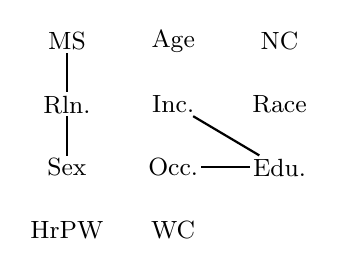
\begin{tikzpicture}
	\begin{scope}[xscale=0.9]
		\tikzstyle{every node}=[align=center, inner sep=1pt]
		\node (ms) at (0, 0) {\small{MS}};
		\node (rln) at (0, -0.8) {Rln.};
		\node (sex) at (0, -1.6) {Sex};
		\node (hrpw) at (0, -2.4) {HrPW};

		\node (age) at (1.5, 0) {Age};
		\node (inc) at (1.5, -0.8) {Inc.};
		\node (occ) at (1.5, -1.6) {Occ.};
		\node (wc) at (1.5, -2.4) {WC};

		\node (nc) at (3, 0) {NC};
		\node (race) at (3, -0.8) {Race};
		\node (edu) at (3, -1.6) {Edu.};

		\draw [thick] (ms) to (rln);
		\draw [thick] (rln) to (sex);
		\draw [thick] (inc) to (edu);
		\draw [thick] (occ) to (edu);
	\end{scope}
	\end{tikzpicture}

	% PC algorithm MI test 800 samples
	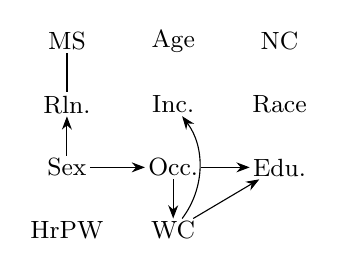
\begin{tikzpicture}
	\begin{scope}[xscale=0.9]
		\tikzstyle{every node}=[align=center, inner sep=1pt]
		\node (ms) at (0, 0) {MS};
		\node (rln) at (0, -0.8) {Rln.};
		\node (sex) at (0, -1.6) {Sex};
		\node (hrpw) at (0, -2.4) {HrPW};

		\node (age) at (1.5, 0) {Age};
		\node (inc) at (1.5, -0.8) {Inc.};
		\node (occ) at (1.5, -1.6) {Occ.};
		\node (wc) at (1.5, -2.4) {WC};

		\node (nc) at (3, 0) {NC};
		\node (race) at (3, -0.8) {Race};
		\node (edu) at (3, -1.6) {Edu.};

		\draw [thick] (ms) to (rln);
		\draw [-{Stealth}] (sex) to (rln);
		\draw [-{Stealth}] (sex) to (occ);
		\draw [-{Stealth}] (occ) to (wc);
		\draw [-{Stealth}] (occ) to (edu);
		\draw [-{Stealth}] (wc) to (edu);
		\draw [-{Stealth}] (wc) to[bend right=40] (inc);
	\end{scope}
	\end{tikzpicture}

	% PC algorithm Q3 test 400 samples
	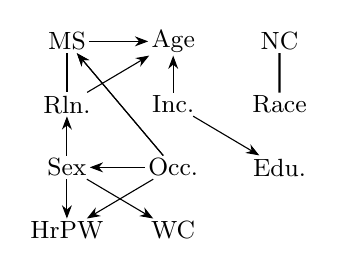
\begin{tikzpicture}
	\begin{scope}[xscale=0.9]
		\tikzstyle{every node}=[align=center, inner sep=1pt]
		\node (ms) at (0, 0) {MS};
		\node (rln) at (0, -0.8) {Rln.};
		\node (sex) at (0, -1.6) {Sex};
		\node (hrpw) at (0, -2.4) {HrPW};

		\node (age) at (1.5, 0) {Age};
		\node (inc) at (1.5, -0.8) {Inc.};
		\node (occ) at (1.5, -1.6) {Occ.};
		\node (wc) at (1.5, -2.4) {WC};

		\node (nc) at (3, 0) {NC};
		\node (race) at (3, -0.8) {Race};
		\node (edu) at (3, -1.6) {Edu.};

		\draw [thick] (ms) to (rln);
		\draw [-{Stealth}] (sex) to (rln);
		\draw [-{Stealth}] (sex) to (hrpw);
		\draw [-{Stealth}] (sex) to (wc);
		\draw [-{Stealth}] (ms) to (age);
		\draw [-{Stealth}] (rln) to (age);

		\draw [-{Stealth}] (inc) to (age);
		\draw [-{Stealth}] (inc) to (edu);
		\draw [-{Stealth}] (occ) to (sex);
		\draw [-{Stealth}] (occ) to (hrpw);
		\draw [-{Stealth}] (occ) to (ms);
		\draw [-{Stealth}] (occ) to (ms);

		\draw [thick] (nc) to (race);
	\end{scope}
	\end{tikzpicture}

	% PC algorithm Q3 test 400 samples
	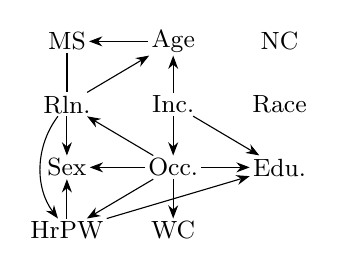
\begin{tikzpicture}
	\begin{scope}[xscale=0.9]
		\tikzstyle{every node}=[align=center, inner sep=1pt]
		\node (ms) at (0, 0) {MS};
		\node (rln) at (0, -0.8) {Rln.};
		\node (sex) at (0, -1.6) {Sex};
		\node (hrpw) at (0, -2.4) {HrPW};

		\node (age) at (1.5, 0) {Age};
		\node (inc) at (1.5, -0.8) {Inc.};
		\node (occ) at (1.5, -1.6) {Occ.};
		\node (wc) at (1.5, -2.4) {WC};

		\node (nc) at (3, 0) {NC};
		\node (race) at (3, -0.8) {Race};
		\node (edu) at (3, -1.6) {Edu.};

		\draw [thick] (ms) to (rln);
		\draw [-{Stealth}] (rln) to (sex);
		\draw [-{Stealth}] (rln) to[bend right=40] (hrpw);
		\draw [-{Stealth}] (rln) to (age);
		\draw [-{Stealth}] (hrpw) to (sex);
		\draw [-{Stealth}] (hrpw) to (edu);
		
		\draw [-{Stealth}] (age) to (ms);
		\draw [-{Stealth}] (inc) to (age);
		\draw [-{Stealth}] (inc) to (occ);
		\draw [-{Stealth}] (inc) to (edu);
		\draw [-{Stealth}] (occ) to (rln);
		\draw [-{Stealth}] (occ) to (sex);
		\draw [-{Stealth}] (occ) to (hrpw);
		\draw [-{Stealth}] (occ) to (wc);
		\draw [-{Stealth}] (occ) to (edu);
	\end{scope}
	\end{tikzpicture}

	% Hill Climb with BIC Score Q3 test 400 samples
	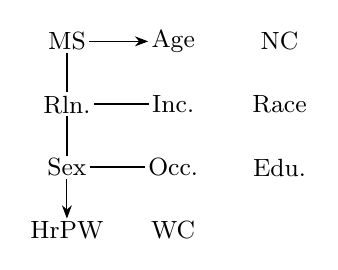
\begin{tikzpicture}
	\begin{scope}[xscale=0.9]
		\tikzstyle{every node}=[align=center, inner sep=1pt]
		\node (ms) at (0, 0) {MS};
		\node (rln) at (0, -0.8) {Rln.};
		\node (sex) at (0, -1.6) {Sex};
		\node (hrpw) at (0, -2.4) {HrPW};

		\node (age) at (1.5, 0) {Age};
		\node (inc) at (1.5, -0.8) {Inc.};
		\node (occ) at (1.5, -1.6) {Occ.};
		\node (wc) at (1.5, -2.4) {WC};

		\node (nc) at (3, 0) {NC};
		\node (race) at (3, -0.8) {Race};
		\node (edu) at (3, -1.6) {Edu.};

		\draw [thick] (ms) to (rln);
		\draw [thick] (rln) to (sex);
		\draw [-{Stealth}] (sex) to (hrpw);

		\draw [-{Stealth}] (ms) to (age);
		\draw [thick] (rln) to (inc);
		\draw [thick] (sex) to (occ);
	\end{scope}
	\end{tikzpicture}

	% Hill Climb with BIC Score Q3 test 800 samples
	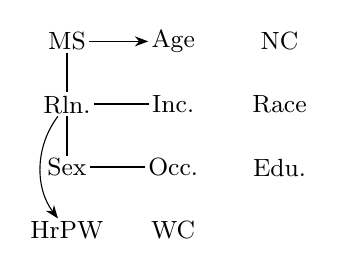
\begin{tikzpicture}
	\begin{scope}[xscale=0.9]
		\tikzstyle{every node}=[align=center, inner sep=1pt]
		\node (ms) at (0, 0) {MS};
		\node (rln) at (0, -0.8) {Rln.};
		\node (sex) at (0, -1.6) {Sex};
		\node (hrpw) at (0, -2.4) {HrPW};

		\node (age) at (1.5, 0) {Age};
		\node (inc) at (1.5, -0.8) {Inc.};
		\node (occ) at (1.5, -1.6) {Occ.};
		\node (wc) at (1.5, -2.4) {WC};

		\node (nc) at (3, 0) {NC};
		\node (race) at (3, -0.8) {Race};
		\node (edu) at (3, -1.6) {Edu.};

		\draw [thick] (ms) to (rln);
		\draw [thick] (rln) to (sex);
		\draw [-{Stealth}] (rln) to[bend right=40] (hrpw);

		\draw [-{Stealth}] (ms) to (age);
		\draw [thick] (rln) to (inc);
		\draw [thick] (sex) to (occ);
	\end{scope}
	\end{tikzpicture}
\end{document}
